\documentclass{article}
\usepackage{german}
\usepackage[latin1]{inputenc}
\usepackage{a4wide}
\usepackage{amssymb}
\usepackage{fancyvrb}
\usepackage{alltt}
\usepackage{epsfig}


\renewcommand{\labelenumi}{(\alph{enumi})}
\renewcommand{\labelenumii}{\arabic{enumii}.}

\begin{document}
\noindent
{\Large \textbf{Aufgaben-Blatt}: Ein Rangier-Problem}
\vspace{0.5cm}


\noindent
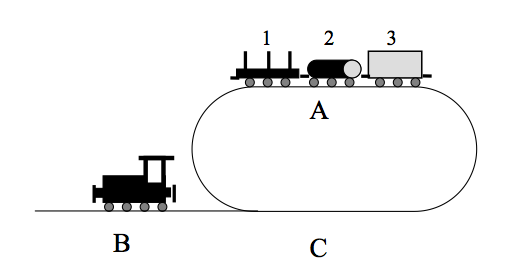
\epsfig{file=rangierProblem, scale=0.8}

\noindent
Auf dem Gleis-Abschnitt A befinden befinden sich drei Waggons, die wir mit 1, 2, 3
bezeichnen.  Auf dem Gleisabschnitt B befindet sich eine Lokomotive, die wir sp�ter mit der
Ziffer 0 bezeichnen.   Ziel ist es, die
Waggons in der Reihenfolge 3, 1, 2 auf dem Gleis-Abschnitt C abzustellen.  Die Lokomotive
soll am Schluss wieder auf den Gleis-Abschnitt B zur�ckfahren.  Die Lokomotive kann die Waggons in
beliebiger Reihenfolge an und abkoppeln.  Beim Rangieren ist es erlaubt, dass die
Lokomotive gleichzeitig Waggons vorne und hinten anh�ngt.

Schreiben Sie ein \textsc{Setl2}-Programm, dass die gestellte Aufgabe l�st.  
Laden Sie dazu von meiner Seite das Programm
\\[0.2cm]
\hspace*{1.3cm}
\texttt{\symbol{126}stroetma/Logic/SetlX/rangier-frame.stlx}
\\[0.2cm]
herunter und bearbeiten Sie die folgenden Teilaufgaben.

\begin{enumerate}
\item Definieren Sie in Zeile 69 eine Funktion \texttt{toList} so, dass f�r eine Menge
      $s$ der Aufruf $\textsl{toList}(s)$ die Menge aller Listen berechnet, deren Elemente
      aus $s$ sind und die jedes Element aus $s$ genau einmal enthalten.  Beispielsweise
      soll der Aufruf $\mathtt{toList}(\{1,2,3\})$ das Ergebnis
      \\[0.2cm]
      \hspace*{1.3cm}
      $\{[1, 2, 3], [1, 3, 2], [2, 1, 3], [2, 3, 1], [3, 1, 2], [3, 2, 1]\}$
      \\[0.2cm]
      liefern.
\item Definieren Sie in Zeile 78 eine Funktion \texttt{reverse} so, dass f�r eine Liste 
      $l$ der Aufruf $\mathtt{reverse}(l)$ eine Liste berechnet, in der die Elemente von
      $l$ in umgekehrter Reihenfolge auftreten.  Beispielsweise soll der Aufruf 
      $\mathtt{reverse}([1,2,3])$ als Ergebnis die Liste $[3,2,1]$ zur�ck geben.
\item Definieren Sie in Zeile 86 eine Prozedur \texttt{inverse} so, dass der Aufruf
      $\mathtt{inverse}(R)$ f�r eine bin�re Relation $R$ die Relation $R^{-1}$ berechnet.
      Beispielsweise soll gelten:
      \begin{verbatim}
      inverse({ ["a", 1], ["b", 2] }) = {[1, "a"], [2, "b"]}.
      \end{verbatim}
\pagebreak

\item Wir stellen die Waggons durch die Ziffern 1, 2 und 3 dar, die Lokomotive wird durch
      0 dargestellt.

      Definieren Sie in Zeile 98 die Menge \texttt{partitions} so, dass diese Menge alle
      Tripel der Form
      \\[0.2cm]
      \hspace*{1.3cm}
      $\langle a, b, c \rangle$
      \\[0.2cm]
      enth�lt, f�r die die Menge $\{ a, b, c \}$ eine Partition der Menge $\{0,1,2,3\}$
      ist.
\item Wir stellen Situationen durch Listen der Form
      \\[0.2cm]
      \hspace*{1.3cm}
      $[ la, lb, lc ]$
      \\[0.2cm]
      dar.  Dabei ist $la$ die Liste der Waggons auf dem Gleis A, $lb$ ist die Liste der
      Waggons auf dem Gleis $lb$ und $lc$ ist die Liste der Waggons auf dem Gleis C.
      
      Berechnen Sie in Zeile 105 die Menge aller Situationen.
\item Berechnen Sie in Zeile 118 die Menge aller Transitionen, in denen die Lokomotive vom
      Gleis A nach Osten zum Gleis C f�hrt.
\item Berechnen Sie in Zeile 133 die Menge aller Transitionen, in denen die Lokomotive vom
      Gleis A nach Westen zum Gleis C f�hrt.
\item Berechnen Sie in Zeile 147 die Menge aller Transitionen, in denen die Lokomotive vom
      Gleis C zum Gleis A f�hrt.  Ber�cksichtigen Sie dabei die Symmetrie des Problems.
\item Berechnen Sie in Zeile 151 die Menge aller Transitionen, in denen die Lokomotive vom
      Gleis B zum Gleis C f�hrt.
\item Berechnen Sie in Zeile 163 die Menge aller Transitionen, in denen die Lokomotive vom
      Gleis C zum Gleis B f�hrt.
\end{enumerate}

\end{document}

%%% Local Variables: 
%%% mode: latex
%%% TeX-master: t
%%% End: 
